% !TEX root = ../chrysalis-report.tex
%
\chapter{Caterpillar}
\label{sec:caterpillar}

One of the tasks of our project was to analyze a system similar to CHRYSALIS and compare it to our project. A project called Caterpillar has been chosen for comparison. In this chapter we give an overview of different versions of Caterpillar, its architecture and working principles, as well as compare it to CHRYSALIS in terms of performance and features implemented.

\section{General overview}
\label{sec:caterpillar:overview}

Caterpillar is an ethereum-based process model execution system. It is available in two versions: Version 2 is a compilation-based engine. It compiles process models into smart contracts being executed by ethereum blockchain. Version 3 is an interpreter-based engine, the model is processed by an interpreter smart contract, which executes the tasks of the process. It implements the compliance-by-design approach - the parties execute each step of a business process by executing transactions on the blockchain. When a transaction is invoked, the blockchain platform checks the current state of the process and the inputs and outputs of the transaction. The transaction is accepted if and only if it complies with the collaborative process model. This approach is suitable for a scenario, where the level of trust between the parties is low, the impact of non-compliance is high, and conflict resolution is expensive. This scenario is addressed by Caterpillar.

\subsection{BPMN features supported}
\label{sec:caterpillar:overview:bpmn}

Caterpillar supports execution of subprocesses, which are implemented through a smart contract hierarchy in the runtime registry contract. For the types of tasks it supports user tasks, service tasks (with solidity smart contracts implementing service logic) and script tasks (with solidity scripts attached). For the beginning of the process it only supports a plain start event. Moreover, the evaluation of exclusive, parallel and event-based gateways is implemented within caterpillar. The types of events supported are terminate, default, message, signal, error and escalation events. t also supports multi-instance activities, parallel as well as sequential and events attached to the boundary of an activity.

\begin{figure}[hbt]
	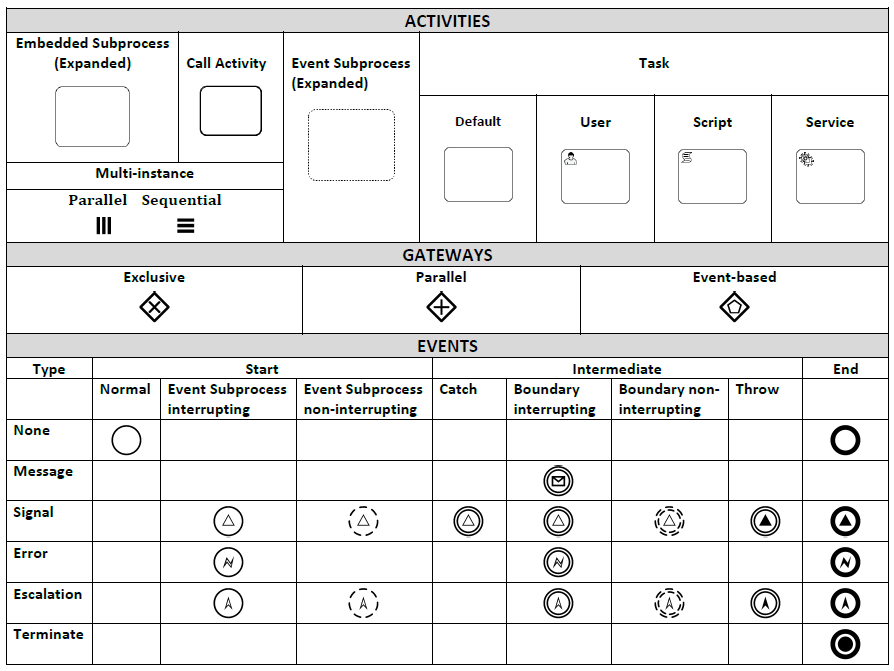
\includegraphics[width=\textwidth]{gfx/caterpillar-bpmn}
	\caption{Overview of the features supported}
	\label{fig:caterpillar:overview:bpmn}
\end{figure}

\subsection{Architecture}
\label{sec:caterpillar:overview:architecture}

In general, the architecture of Caterpillar is similar to this of our project. It consists of three layers - on-chain layer, responsible for deployment and execution of processes, backend layer, responsible for processing bpmn-models and interacting with the blockchain and frontend layer, providing a user interface (except for version 3, which does not have the frontend layer). The only difference on this level is that the backend layer is implemented as a REST-server and not a library (which allows users to interact with the version 3 of caterpillar even without the web application).

The On-chain layer supports the execution of smart contracts that fully encode a set of process models. The events generated by the contracts are recorded and stored in the Ethereum log, which can be accessed from outside the blockchain. The process repository is an off-chain storage, keeping and providing access to BPMN-models, solidity code generated from them (only in version 2), and metadata linking solidity contracts to elements of bpmn-models. The process repository is implemented on the top of Interplanetary File System (IPFS).

The off-chain runtime layer (referred previously as backend layer) includes tools to compile (only in version 2), deploy and monitor business processes in the blockchain, which allow external applications to interact with the on-chain components and the repository. Finally, the top-most layer incorporates a set of tools for editing process models, packaging process configurations and initiate and monitor execution of process instances.

\begin{figure}[hbt]
	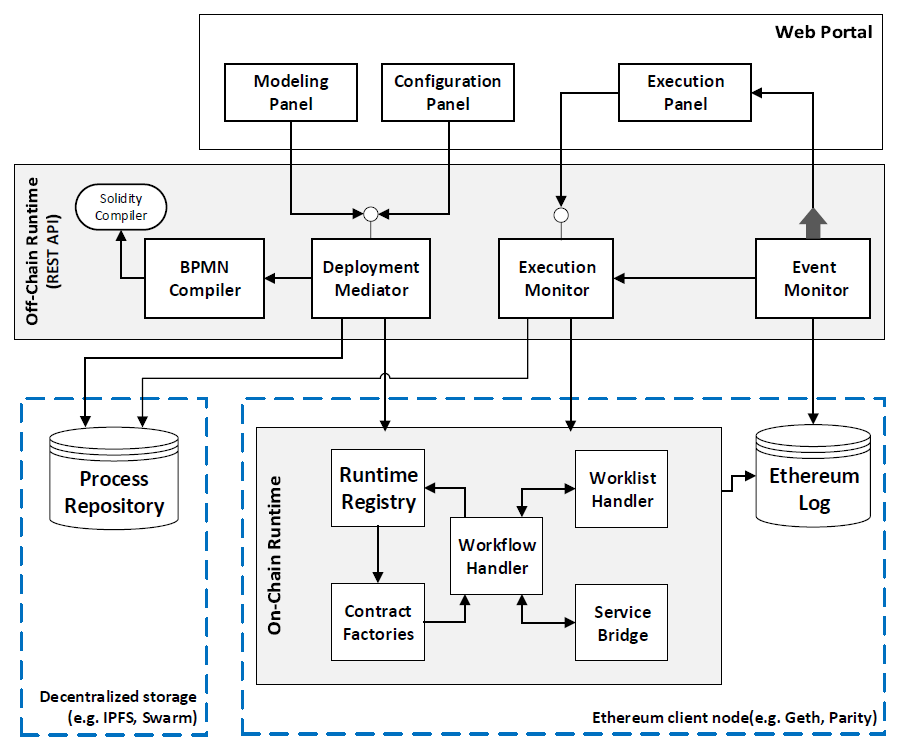
\includegraphics[width=\textwidth]{gfx/caterpillar-architecture}
	\caption{General architecture of Caterpillar}
	\label{fig:caterpillar:overview:architecture}
\end{figure}

\section{Compilation engine}
\label{sec:caterpillar:v2}

The version 2 of Caterpillar provides an engine based on the compilation of BPMN-models into solidity smart contracts. In this section we will give an overview of the compilation process as well as the smart contract structure of this version of Caterpillar.

\subsection{Compilation process}
\label{sec:caterpillar:v2:compilation}
For each process model uploaded Caterpillar V2 generates a set of solidity smart contracts. The compilation is conducted in two steps. On the first step, the solidity code for the process contracts is generated, as well as additional metadata, called the compilation dictionary, which is used for monitoring processes. It is a data structure which maps the elements of the source model to the generated code. This information includes the name of the contract method associated with an activity, a unique integer index assigned to each element, as well as the element type.

On the second step, the generated smart contracts are put together, as well as pre-existing contracts, i.e attached to the service tasks. These contracts are then passed to the solidity compiler, which produces EVM-bytecode and ABI definitions for each contract, that are needed for deploying smart contracts on Ethereum. These definitions are later used by off-chain components to interact with the contracts and trigger their execution. Artifacts of the compilation are stored in the process repository.

\begin{figure}[hbt]
	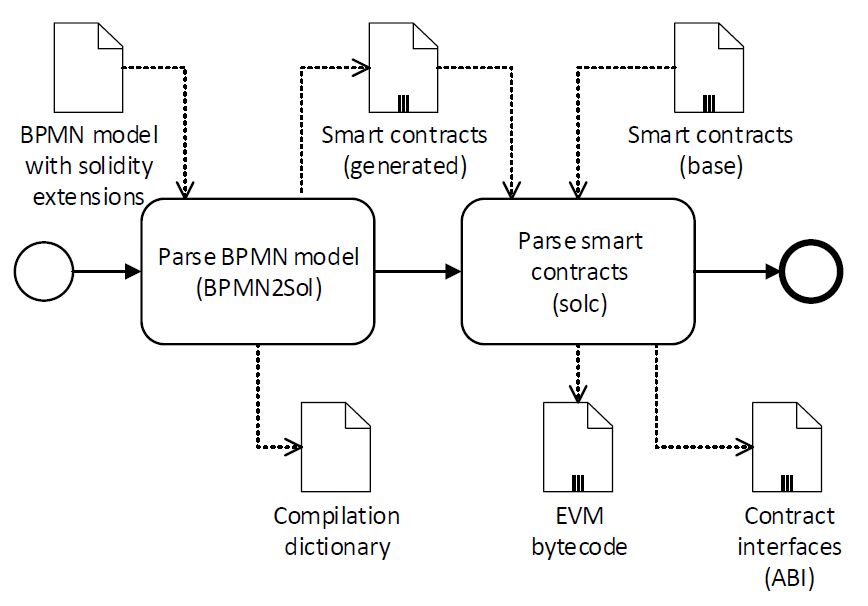
\includegraphics[width=\textwidth]{gfx/caterpillar-compilation-process}
	\caption{Caterpillar V2 compilation process}
	\label{fig:caterpillar:v2:compilation}
\end{figure}

\subsection{Smart contracts}
The contract that is deployed at the start of the application is the process registry contract. It keeps track of the deployed process models, their corresponding contracts, started process instances and their execution states. It also stores the subprocess hierarchy by keeping links between smart contract bundles associated with each process therein.

The contracts generated for each of the process models implement interfaces AbstractProcess, AbstractFactory and AbstractWorklist. The contracts implementing AbstractProcess interface contain information on the process structure, methods implementing execution of different process model elements, including firing and handling events. It also contains a reference to the parent process if it exists, as well as a reference to the worklist contract. The contracts implementing AbstractWorklist interface implemement data perspective of the process model execution. They store process variables with association to the model elements.
The contracts implementing AbstractFactory interface contain logic relating to creating and starting execution of new process instances. They are called from the process registry on instantiation and from the process contract on execution.

\begin{figure}[hbt]
	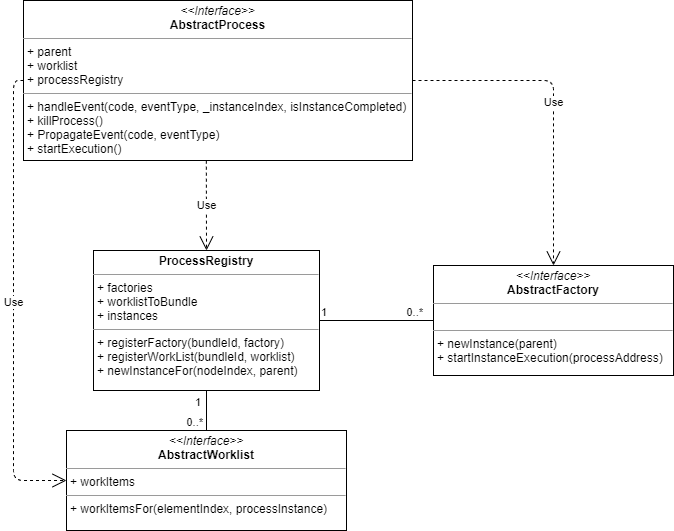
\includegraphics[width=\textwidth]{gfx/caterpillar-compilation-contracts}
	\caption{Structure of the Caterpillar V2 smart contracts}
	\label{fig:caterpillar:v2:contracts}
\end{figure}

\section{Interpretation engine}
\label{sec:caterpillar:v3}

In the version 3 of the caterpillar application, the process execution paradigm was changed significantly. Instead of compiling process models into smart contracts, the models were read and executed by an interpreter contract. In this section we give an overview of this version of caterpillar

\subsection{Interpretation process}
\label{sec:caterpillar:v3:process}

The control flow component stores the information about structure of the process model, its elements and relations. The data is organized in a tree-like structure to implement the subprocess hierarchy. Each node in the tree maps for each enclosed BPMN element the model-related information to be used by the interpreter. As a result, each node is deployed once for each subprocess in the model and is identified by the corresponding address.

The process case factories include the set of contracts to instantiate and start the execution of a business process. Therefore, if a subprocess is linked into the hierarchy, the parent has to store an address of the corresponding factory to instantiate the subprocess.

The data and scripts component implements the data perspective. To implement separate data requirements for each process, smart contracts are compiled from each process model. The scripts related to user/service/script tasks and the conditions to decide the paths in exclusive gateways mostly interact with the process data. Thus, such instructions are also compiled from the model into the contract implementing the data perspective.\\

Bpmn interpreter implements the process execution logic. It keeps no information about any of the process perspectives, but queries data from other components during execution. The runtime handler keeps track of the process instances. The operation of the runtime handler is similar to that of the Caterpillar version 2.

\begin{figure}[hbt]
	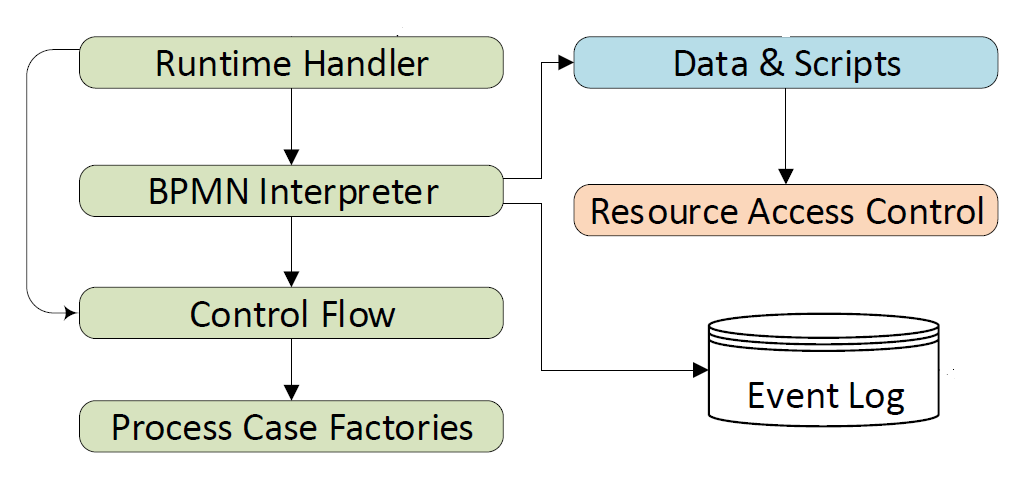
\includegraphics[width=\textwidth]{gfx/caterpillar-interpretation-architecture}
	\caption{General architecture of the V3 on-chain components}
	\label{fig:caterpillar:v3:architecture}
\end{figure}

\subsection{Smart contracts}
\label{sec:caterpillar:v3:contracts}

Aside from the process registry contract discussed in the section regarding Caterpillar v2, the BPMN Interpreter contract is also deployed only once at the start of the application. It contains functions responsible for the execution of process, including execution of activities, throwing and catching events. It also provides an entry point for the off-chain part of the application to interact with the on-chain runtime, initiating most of the actions on it.

During contract instantiation it calls the appropriate contract imlementing IFactory interface, which contains logic relevant for creating process cases/instances. The IData contract is deployed for each process case/instance and is used by the interpreter to handle data perspective during the process element execution. It also keeps the information on the process state (started activities field) and a link to its parent in the subprocess hierarchy.

The IFlow contract is deployed for each process model and contains the data relevant to the hierarchy of subprocesses (each deployed IFlow contract is a node in a subprocess tree), control flow perspective, as well as created IData instances. It is also linked to the interpreter and uses its functionality for addition of newly created IData instances.

\begin{figure}[hbt]
	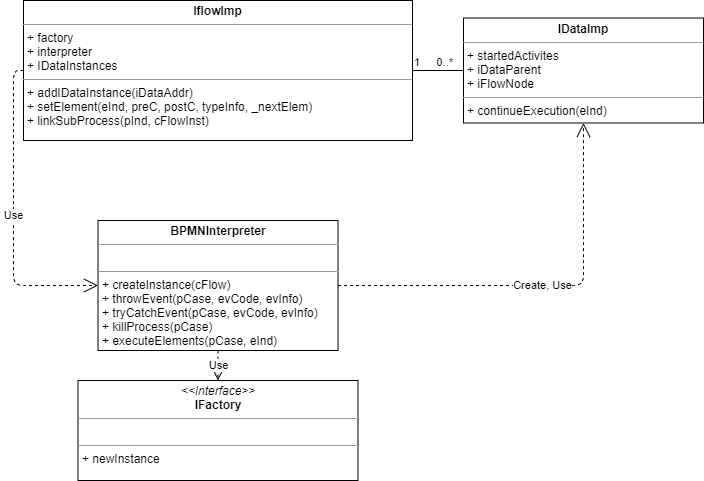
\includegraphics[width=\textwidth]{gfx/caterpillar-interpretation-contracts}
	\caption{Structure of the V3 smart contracts}
	\label{fig:caterpillar:v3:contacts}
\end{figure}

\section{Evaluation and comparison}
\label{sec:caterpillar:eval}

In this section we compare Caterpillar and CHRYSALIS in terms of the features supported and project architecture, as well as evaluate the performance of Caterpillar and Chrysalis on the process deployment and instantiation

\subsection{Comparison}
\label{sec:caterpillar:eval:comp}

Caterpillar supports much wider array of BPMN-features: Sub processes, User tasks, Script tasks, Service tasks, events, control flow decisions. Whereas CHRYSALIS only supports execution of plain tasks and evaluation of defferent types of gateways. The business logic layer of Caterpillar is implemented as a REST-service, whereas CHRYSALIS implements it as a library, which works to its disadvantage, since one should integratet it in some other application to use it, and also ensure the library's compatibility with this project, which has already lead to complications during development, when we could not integrate the enzian library, containing logic for interaction with Hyperledger due to the Hyperledger components' incompatibility with the Webpack version used in the web application.

In terms of runtime customization of the blockchain connection parameters CHRYSALIS has a significant advantage, since it allows the user to set the Ethereum node address and account for signing the transaction, whereas in Caterpillar all of these parameters are hardcoded into the application, which makes it less applicable for an actual production environment.

Process deployment and instantiation in CHRYSALIS are done in a single step, which means that for each new process case, one has to redeploy the whole model. Whereas in Caterpillar one can create multiple process instances for each model, thus reducing performance costs.

\begin{table}[hbt]
	\begin{tabular}{|l|l|l|l|l|}
		\hline
		& \begin{tabular}[c]{@{}l@{}}BPMN-feature \\ support\end{tabular}                                                                             & \begin{tabular}[c]{@{}l@{}}Business-logic \\ implementation\end{tabular} & \begin{tabular}[c]{@{}l@{}}Blockchain \\ connection \\ customization\end{tabular} & \begin{tabular}[c]{@{}l@{}}Separate \\ process \\ instantiation\end{tabular} \\ \hline
		Caterpillar & \begin{tabular}[c]{@{}l@{}}Sub processes, \\ User tasks, \\ Script tasks, \\ Service tasks,\\ events,\\ control flow decisions\end{tabular} & REST-service                                                             & No                                                                                & Yes                                                                          \\ \hline
		CHRYSALIS   & \begin{tabular}[c]{@{}l@{}}Plain tasks, \\ control flow decisions\end{tabular}                                                              & Library                                                                  & Yes                                                                               & No                                                                           \\ \hline
	\end{tabular}
	\caption{Summary of comparison between CHRYSALIS and Caterpillar}
	\label{tab:caterpillar:eval:comp}
\end{table}

\subsection{Evaluation}
\label{sec:caterpillar:eval:eval}

As a base for evaluation a simplified version of the process model "Order to cash" from the Caterpillar repository was used. The simplification consisted of eliminating the features not supported by CHRYSALIS, to be able to compare the performance on the same model. As a result, the subprocesses were eliminated from the model replaced by simple tasks. This model is chosen to evaluate the performance on the most basic BPMN processes, namely activity execution and control flow handling with a parallel and merging gateway.

\begin{figure}[hbt]
	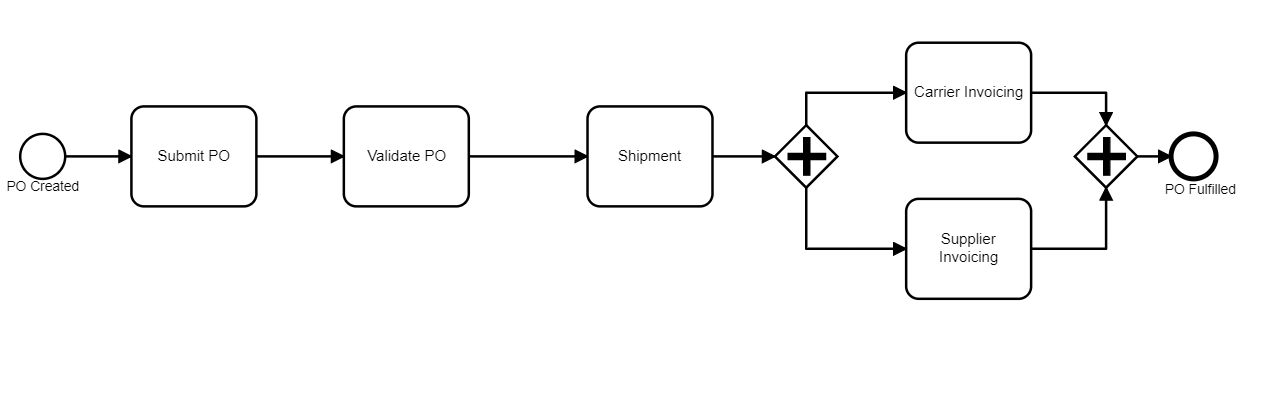
\includegraphics[width=\textwidth]{gfx/caterpillar-eval-model}
	\caption{Model used for evaluation}
	\label{fig:caterpillar:eval:model}
\end{figure}

Gas consumption was used as a performance metric, the process deployment operation process execution were taken into account, since these are the most frequent and the most expensive operations, which dominate in the performance cost. In the result table deployment and instantiation aperations are counted separately for Caterpillar, but in essence they are equivalent to the CHRYSALIS deployment operation, which implicitly does the process case instantiation as well, so to correctly compare the costs of process deployment between Caterpillar and CHRYSALIS one has to take a sum of deployment and instantiation costs for Caterpillar.

\begin{table}[hbt]
	\begin{tabular}{|l|l|l|l|}
		\hline
		& Deployment & Instantiation & Execution            \\ \hline
		Caterpillar V2 & 2015121    & 826808        & $\sim$80834 p. task  \\ \hline
		Caterpillar V3 & 1390012    & 600116        & $\sim$55005 p. task  \\ \hline
		CHRYSALIS      & 3638445    & -             & $\sim$116109 p. task \\ \hline
	\end{tabular}
	\caption{Caterpillar and CHRYSALIS evaluation}
	\label{tab:caterpillar:eval:eval}
\end{table}
As a result of the evaluation one can see, that the performance costs for the Caterpillar interpreter engine are significantly lower than those for Compiler engine of Caterpillar and CHRYSALIS, and that can be explained by the fact that most of the logic, including external entry points is handled by BPMN interpreter, which is deployed only at the start of the application and is not included in this evaluation. The deployed contracts contain only simplest logic for storing process-related information, and giving it to the interpreter upon request.

Compiler engine of Caterpillar seems to perform less costly than CHRYSALIS, but this result is influenced by the model used. Since Caterpillar v2 generates its contracts for each specific model, it can optimize those contracts for the specific model, whereas CHRYSALIS smart contract system is more universal and the same code is deployed for each model. That leads to Caterpillar being more efficient on deployment for relatively small process models, like the one used in the initial evaluation, but with the growth of the model the deployment costs will also grow, whereas for CHRYSALIS these costs will remain constant. To prove it, we have deployed models with number of tasks ranging from 5 to 30 with a step of 5, and measured the costs. The resulting measurements confirm our prediction - deployment costs for Caterpillar V2 grow in linear dependence with the size of the model, and deployment costs for Caterpillar V3 and CHRYSALIS remain constant.

\begin{figure}[hbt]
	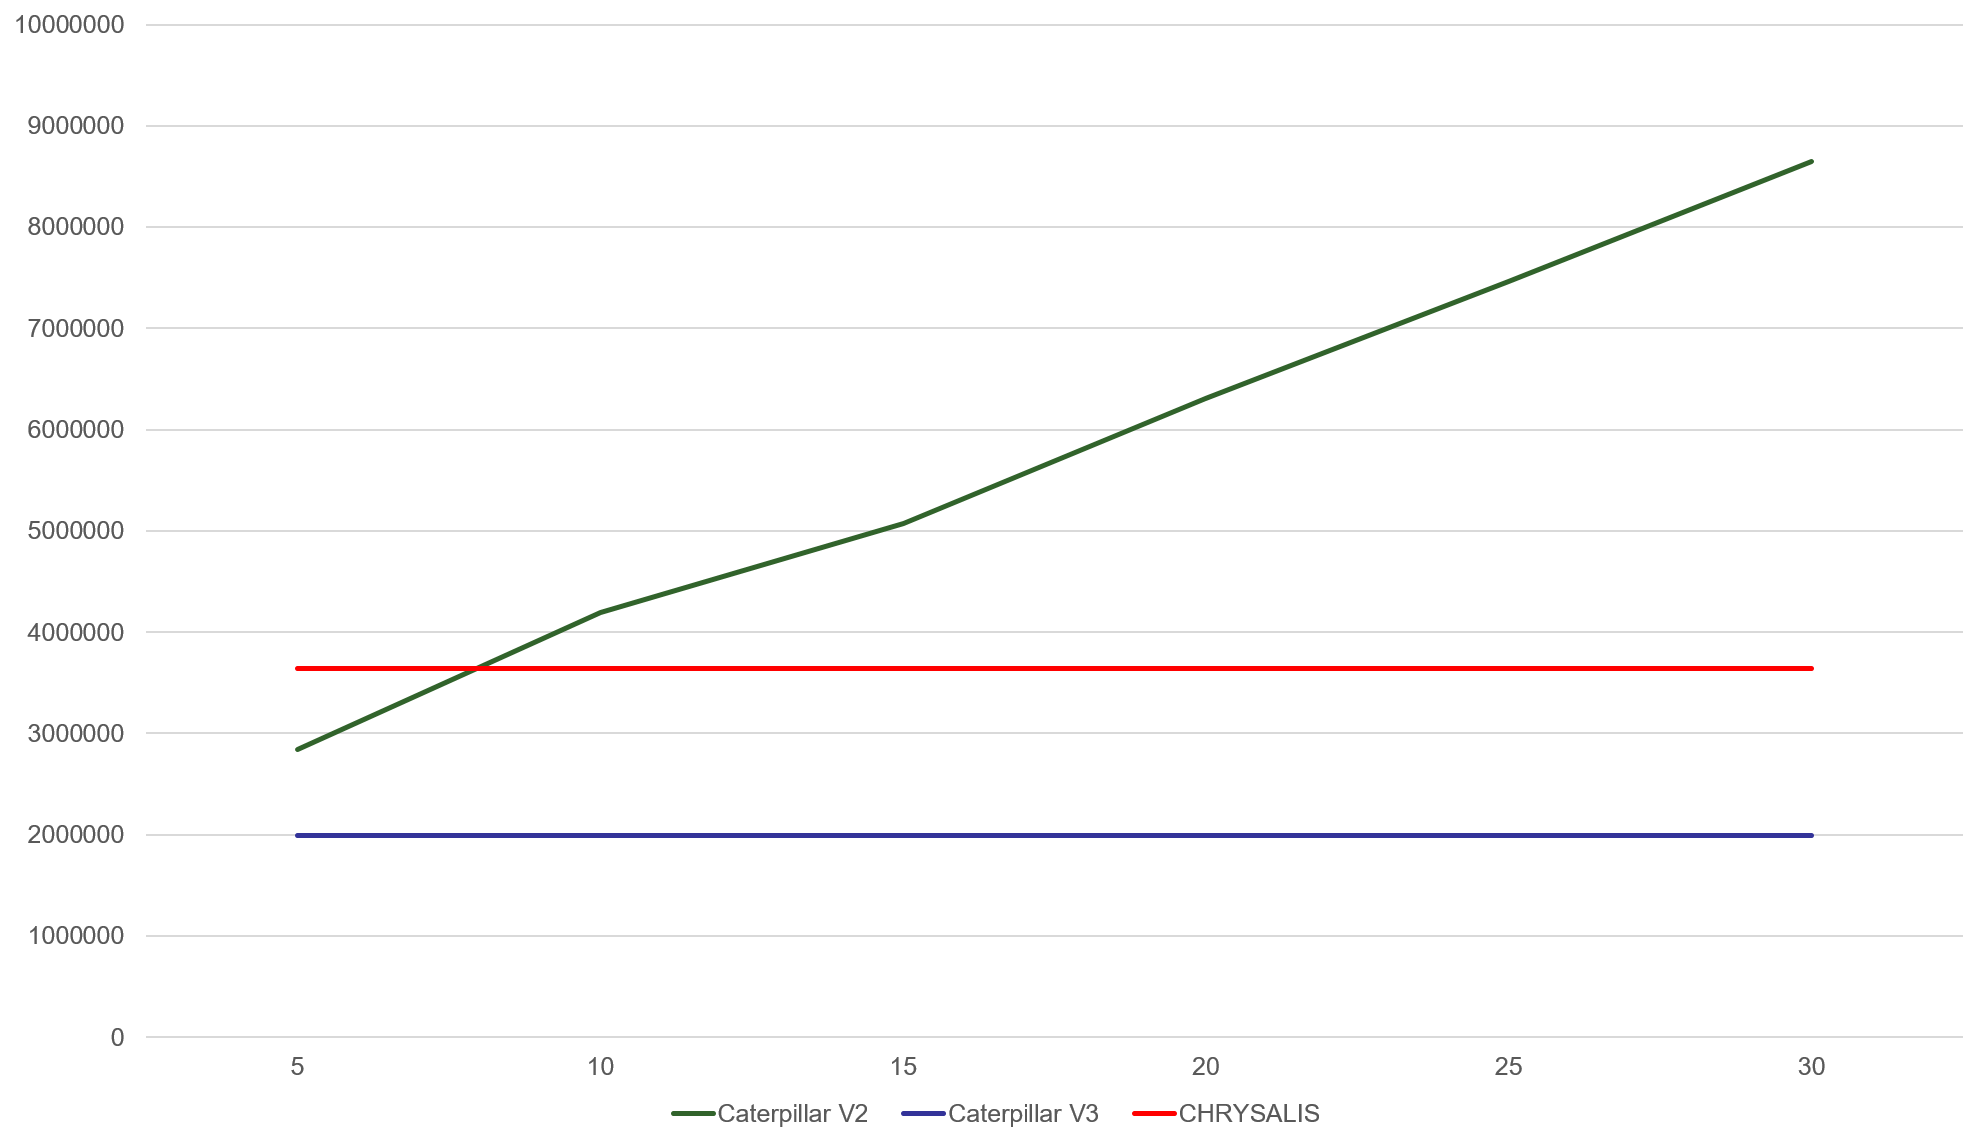
\includegraphics[width=\textwidth]{gfx/caterpillar-eval-graph}
	\caption{Deployment costs in relation to model size}
	\label{fig:caterpillar:eval:graph}
\end{figure}

